\documentclass[twoside]{article}

\usepackage{cite}
\usepackage{listings}
\usepackage{tabularx}

\usepackage[sc]{mathpazo} % Use the Palatino font
\usepackage[OT1]{fontenc} % Use 8-bit encoding that has 256 glyphs
\usepackage[utf8]{inputenc}
\linespread{1.05} % Line spacing - Palatino needs more space between lines
\usepackage{microtype} % Slightly tweak font spacing for aesthetics
\usepackage{graphicx}

\usepackage[hmarginratio=1:1,top=32mm,columnsep=20pt]{geometry} % Document margins
\usepackage{multicol} % Used for the two-column layout of the document
\usepackage[hang, small,labelfont=bf,up,textfont=it,up]{caption} % Custom captions under/above floats in tables or figures
\usepackage{booktabs} % Horizontal rules in tables
\usepackage{float} % Required for tables and figures in the multi-column environment - they need to be placed in specific locations with the [H] (e.g. \begin{table}[H])
\usepackage{hyperref} % For hyperlinks in the PDF

\usepackage{lettrine} % The lettrine is the first enlarged letter at the beginning of the text
\usepackage{paralist} % Used for the compactitem environment which makes bullet points with less space between them

\usepackage{abstract} % Allows abstract customization
\renewcommand{\abstractnamefont}{\normalfont\bfseries} % Set the "Abstract" text to bold
\renewcommand{\abstracttextfont}{\normalfont\small\itshape} % Set the abstract itself to small italic text

\usepackage{titlesec} % Allows customization of titles
\renewcommand\thesection{\Roman{section}} % Roman numerals for the sections
\renewcommand\thesubsection{\Roman{subsection}} % Roman numerals for subsections
\titleformat{\section}[block]{\large\scshape\centering}{\thesection.}{1em}{} % Change the look of the section titles
\titleformat{\subsection}[block]{\large}{\thesubsection.}{1em}{} % Change the look of the section titles

\usepackage{amsmath}

\title{\vspace{-15mm}\fontsize{24pt}{10pt}\selectfont\textbf{Some nice title}}

\date{}

\author{
  \large
  \textsc{Ville Toiviainen}\\[2mm]
  \tt ville.j.toiviainen@aalto.fi \\[2mm]
  \textsc{Antti Partanen}\\[2mm]
  \tt antti.partanen@aalto.fi \\[2mm]
}

%----------------------------------------------------------------------------------------

\begin{document}

\maketitle % Insert title

%----------------------------------------------------------------------------------------
%	ABSTRACT
%----------------------------------------------------------------------------------------

\begin{abstract}
  \noindent{}


\end{abstract}

%----------------------------------------------------------------------------------------
%	ARTICLE CONTENTS
%----------------------------------------------------------------------------------------

\begin{multicols}{2} % Two-column layout throughout the main article text

  \section{Introduction}
  \label{sec:introduction}
  In recent year biggest development steps in reinforced learning have been related to solutions that use deep learning. The major step was taken by DeepMind team that used Deep Q-Networks with Atari games. For this reason, we wanted to experience with Deep Q-Networks in Atari environments. For comparison, we implemented Policy gradient, which has been an interesting topic of research lately as well.

\subsection{Reinforced Learning}
In reinforced learning, the algorithm learns the environment by interacting with it. It’s a goal-driven way to learn - good actions are often rewarded and bad ones receive a penalty. No wonder that games are a very popular way to test reinforced learning.
To learn the algorithm needs to evaluate its performance - how good decision it was to choose this action? In many cases, the algorithm takes multiple actions before it ends up in the terminal state. This forms multiple distinct action-state sequences that have their own rewards. Markov decision process (MDP) is an important property which means that these sequences can be used as a state. In Q-learning, another important property is that when iteration count approaches to infinity Q-function approaches the optimal Q*. This formalism is called Bellman equation. \cite{mnih2015human}

\subsection{Q-Learning}
In Q-Learning the model learns to estimate the optimal action-value function defined in function \ref{eq:qlearning}.
\begin{equation}
    \label{eq:qlearning}
    Q*(s,a) = \mathbf{E}_{s'} \Big[ r + \gamma \max_{a'} Q*(s',a')|s, a \Big]
\end{equation}
If the environment fulfills the requirements of MDP and Bellman equation eventually when $i \rightarrow \infty$, $Q \rightarrow Q*$.
Q-Learning is an off-policy algorithm which in this case is mandatory since experience replay is used to boost the learning. Experience replay is explained in methods and experiments section. \cite{mnih2015human} \cite{rlintroduction}

\subsection{Deep Learning}
Deep Learning is an area of machine learning that uses deep neural networks for the learning task. ”Neural networks have emerged as an important tool for classification. The recent vast research activities in neural classification have established that neural networks are a promising alternative to various conventional classification methods. The advantage of neural networks lies in the following theoretical aspects. First, neural networks are data-driven self- adaptive methods in that they can adjust themselves to the data without any explicit specification of functional or distributional form for the underlying model. Second, they are universal functional approximators in that neural networks can approximate any function with arbitrary accuracy \cite{zhang2000neural}.” This powerful way to approximate function is especially useful in reinforced learning where a system needs to learn to approximate very complex environment and finding the true optimal function can be too demanding time-wise and computationally.

\subsection{OpenAI Gym}
OpenAI Gym is a toolkit for testing and training reinforcement learning algorithms. OpenAI Gym provides “environments” or test problems that have a generalized interface that allows people to write reinforcement algorithms to try to solve those problems. OpenAI Gym includes different environments, ranging from different games (in 2D and 3D) to various algorithmic problems.

One of the environment we used was Cart Pole. Cart Pole environment outputs four values: cart position, cart velocity, pole velocity and pole velocity at the top. These four values are given as an input to the neural network. Network’s outputs are two values - Q-values for actions “go left” and “go right”. The maximum number of actions to take is 200. Every action is rewarded with a reward of +1.







  \section{Methods}
  \label{sec:methods}
  \subsection{Deep Q-Networks}
Deep Q-networks approximate Q-function in Q-learning with neural networks. Value from the action-value function is compared to the correct one with the equation \ref{eq:qlearning}. This way network eventually learns the optimal Q-function. Backpropagation can be done after every action or after a number of iterations. The later makes the learning process smoother. \cite{mnih2015human}

\begin{equation}
    y_j = \left\{
        \begin{array}{l}
            r_j, \:\: if\:j + 1\:is\:terminal \\
            r_j + \gamma \max_{a'} Q^*(\phi_{j+1},a'; \theta^*)
        \end{array}
    \right.
\end{equation}
\begin{equation}
    \label{eq:msedqn}
    Loss = (y_j - Q(\phi_j, a_j; \theta))^2
\end{equation}

In many environments, actions that are next to each other have a strong correlation. If the minibatches used in training would only contain correlated samples learning would be slow and even ineffective. Experience replay is a technique that solves this problem. Previous state-action pairs are stored in the memory and these pairs are used in the training randomly. This means that minibatches contain a lot of samples from different state-action pairs observed from the environment. This removes the strong correlation and makes the learning more efficient and smoother. Only requirement is that the learning algorithm is off-policy, which Q-learning is.

One dilemma in reinforced learning is exploration vs exploitation. In Q-learning, the model takes the action that has the highest reward unless there’s stochasticity in the process. In DQN $\epsilon$-greedy is used for that.

\subsection{Policy Gradient}

\subsection{Cart Pole}
Cart Pole environment outputs four values: cart position, cart velocity, pole velocity and pole velocity at the top. These four values are given as an input to the neural network. Network’s outputs are two values - Q-values for actions “go left” and “go right”. The maximum number of actions to take is 200. Every action is rewarded with a reward of +1.

  \section{Experiments}
  \label{sec:experiments}
  In this section we cover different experiments that we did. With DQN we experienced with different network architectures, $\epsilon$-greedy strategies and experience replay strategies.

\subsection{Different Network architectures}
We used feedforward neural networks as our deep learning method. Input and output sizes are determin by the environment - e.g Cart Pole has 2 input values and two output values. Everything between can be altered. We decided to limit our network depth two maximum layer size of two. That meant that we experienced with networks that contained one or two layers. Neuron count in layers the second architectural thing that we altered. Three experienced architectures are listed in the table \ref{table:nn_arch}.
\begin{table}[H]
    \caption{Different network architectures used with DQN.}
    \centering
    \label{table:nn_arch}
    \scalebox{0.7}{
        \begin{tabular}{lll}
            \multicolumn{2}{r}{Neuron count in} \\
            \cline{2-3}
            Layers & 1st hidden layer & 2nd hidden layer \\
            \hline
            1 & 24 & \\
            2 & 24 & 24 \\
            2 & 24 & 48
        \end{tabular}
    }
\end{table}
In all the experiments activation function was ReLU and loss was measured with mean squered error. Also all the hyperparameters where the same.

\subsection{$\epsilon$-greedy strategies}
Two different linear $\epsilon$-greedy strategies, equation 4 and 5, were tested. In all the cases number of steps ($s$) effected the value with decay ($d$) parameter. Maximum $epsilon_{max}$ value was 1 and minimum $\epsilon_{min}$ 0.01.

\begin{align}
    \epsilon_{min} + (\epsilon_{max} - \epsilon_{min}) * e^{(-\frac{s}{d})} \\
    max \{\epsilon_{min},\:\frac{\epsilon_{max}}{max \{1, (sd)\}} \}
\end{align}

\subsection{Experience replay strategies}
Essential part of DQN is experience replay. The more observations we can store the better \cite{mnih2015human}. Unfortunately storing huge amount of observations introduces memory limits and using huge minibatch sizes means very heavy computations. For this reason we experienced with different Experience replay strategies to learn which could be good enough setup for this problem.

We started with dummy one that included just the last two observations. Second experience contained last 1000 observations and used 64 of those randomly. Third one stored last 100000 observations and used 64 of those randomly.

\subsection{Space Invaders}
Space Invaders is an Atari game which can be played in OpenAI gym with RAM obserations. RAM input only contains 128 features. This means that in this environment input is 128. Output size is the number of actions, which in Space invaders is 6. No other changes are done to the DQN model.

  \section{Results}
  \label{sec:results}
  \subsection{DQN with Cart Pole}
\textbf{Different network architectures} had clearly performance differences. The most simple network that contained one hidden layer and 24 neurons was not able to learn the task in 1000 episodes. From the figure \ref{fig:nn_24} we can see that it was close to reaching the average reward of 200 and it had strong upwards trend in the end. Learning only spiked upwards so the model avoided sudden drops in reward which happened more often with the other architectures.

\begin{figure}[H]
    \centering
    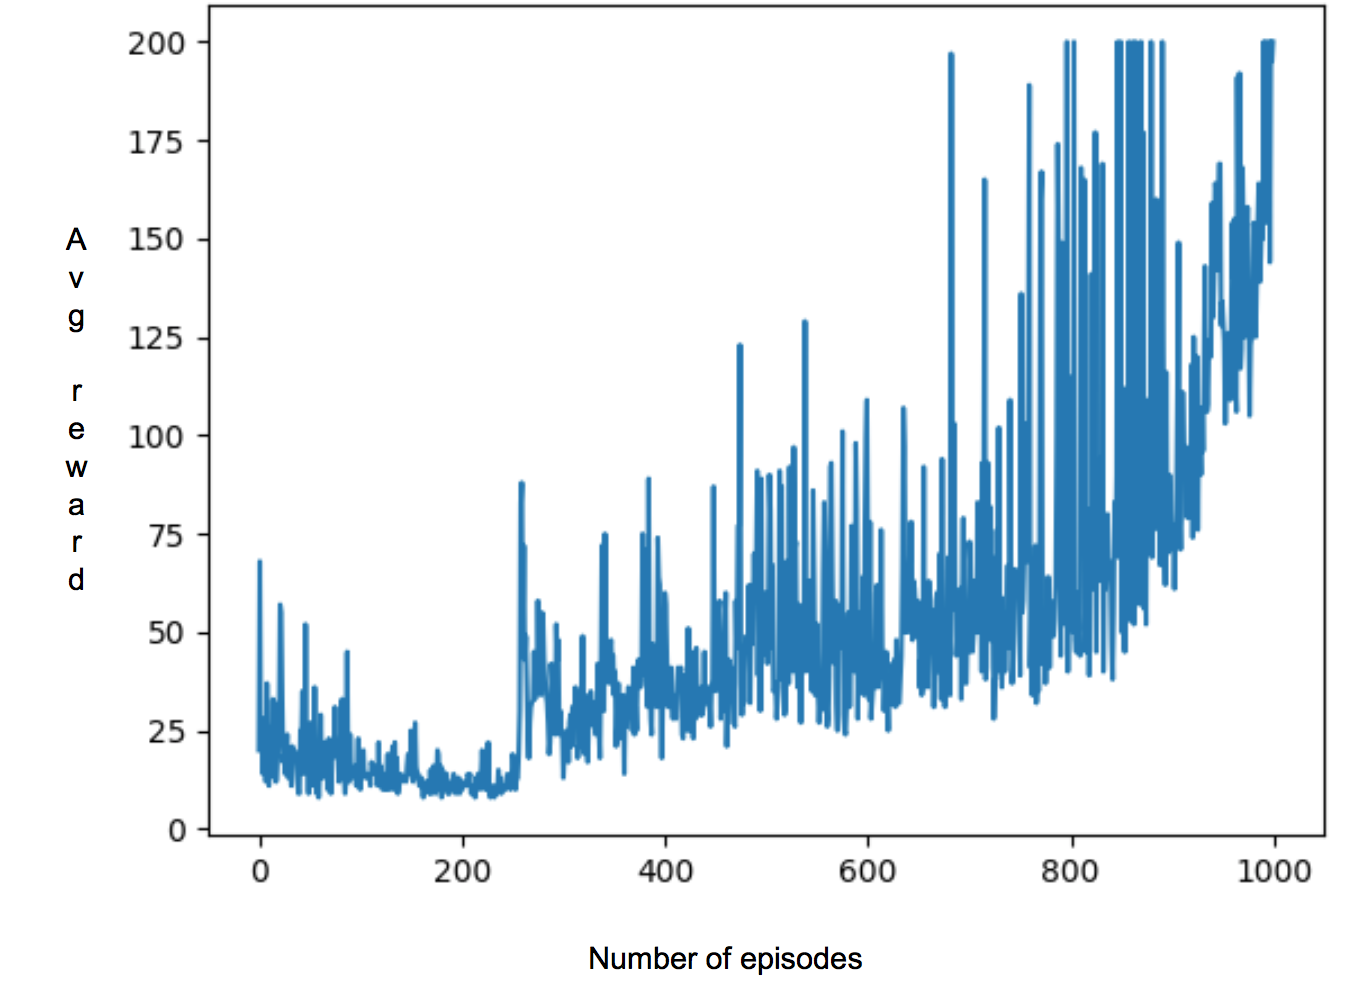
\includegraphics[width=0.4\textwidth]{images/nn_24.png}
    \caption{
    Episode rewards for architecture with one hidden layer with 24 neurons.
    }
    \label{fig:nn_24}
\end{figure}

The two more complex networks learned the task (the average reward was over 195) under 350 episodes. From figures \ref{fig:nn_24_24} and \ref{fig:nn_24_48} we can see that network with 24 neurons in both layers learned the task more generally. It didn't have huge drops in the reward that the more complex network had even after it had multiple successful episodes that achieved the maximum reward.

\begin{figure}[H]
    \centering
    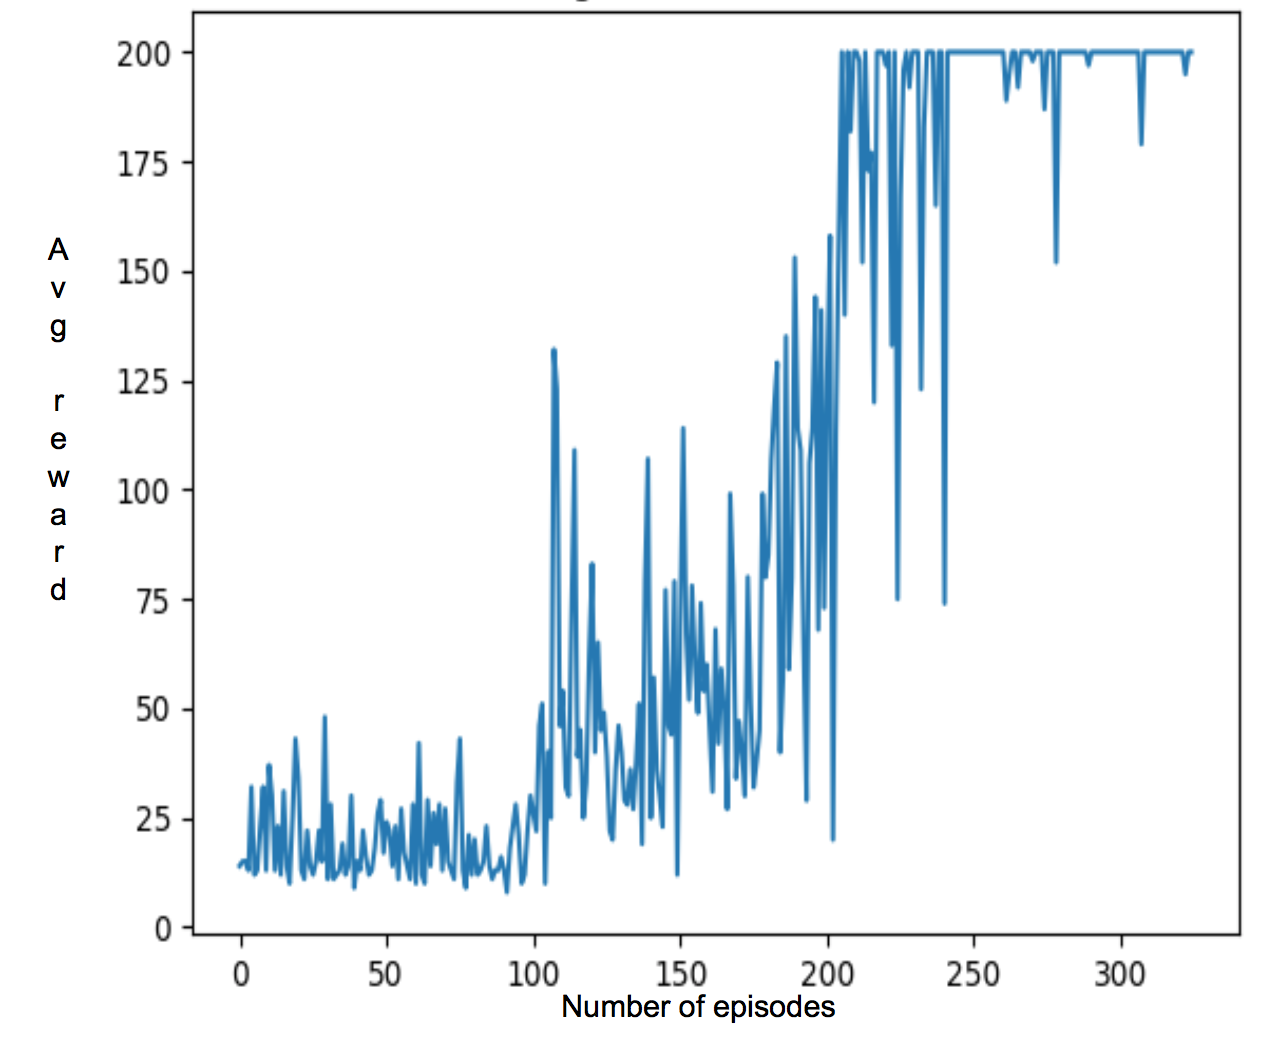
\includegraphics[width=0.4\textwidth]{images/nn_24_24.png}
    \caption{
    Episode rewards for architecture with two hidden layers with 24 neurons.
    }
    \label{fig:nn_24_24}
\end{figure}

\begin{figure}[H]
    \centering
    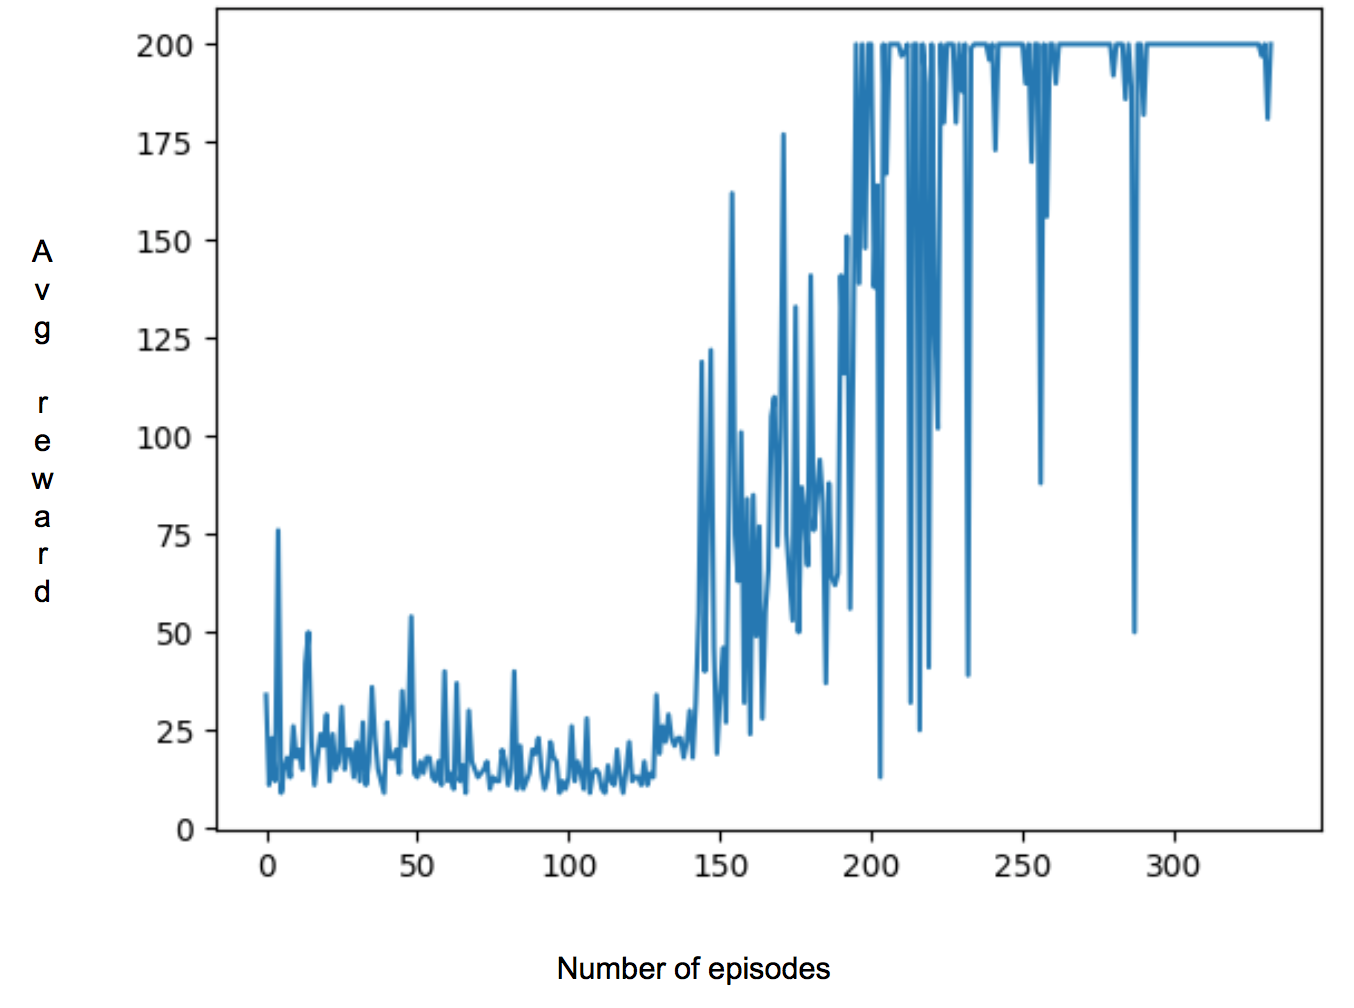
\includegraphics[width=0.4\textwidth]{images/nn_24_48.png}
    \caption{
    Episode rewards for architecture with two hidden layers from which the first had 24 neurons and the second 48.
    }
    \label{fig:nn_24_48}
\end{figure}

\textbf{Different $\epsilon$-greedy strategies} had the results we expected. When the algorithm was not able to explore enough it exploited a strategy that was a local minimum. As a result, the model was not able to reach maximum score.
With really eager $\epsilon$-greedy strategy, where $epsilon$ value was over 0.1 still after 1000 episodes, the model was not able to learn optimal strategy. Reasons are obvious since there is very high probability 0.1 that action is taken randomly. Results for this epsilon we can see from the figure \ref{fig:e-greedy}.
Best $\epsilon$-greedy strategy was achieved with the formula 5 that had the decay of 0.1.

\begin{figure}[H]
    \centering
    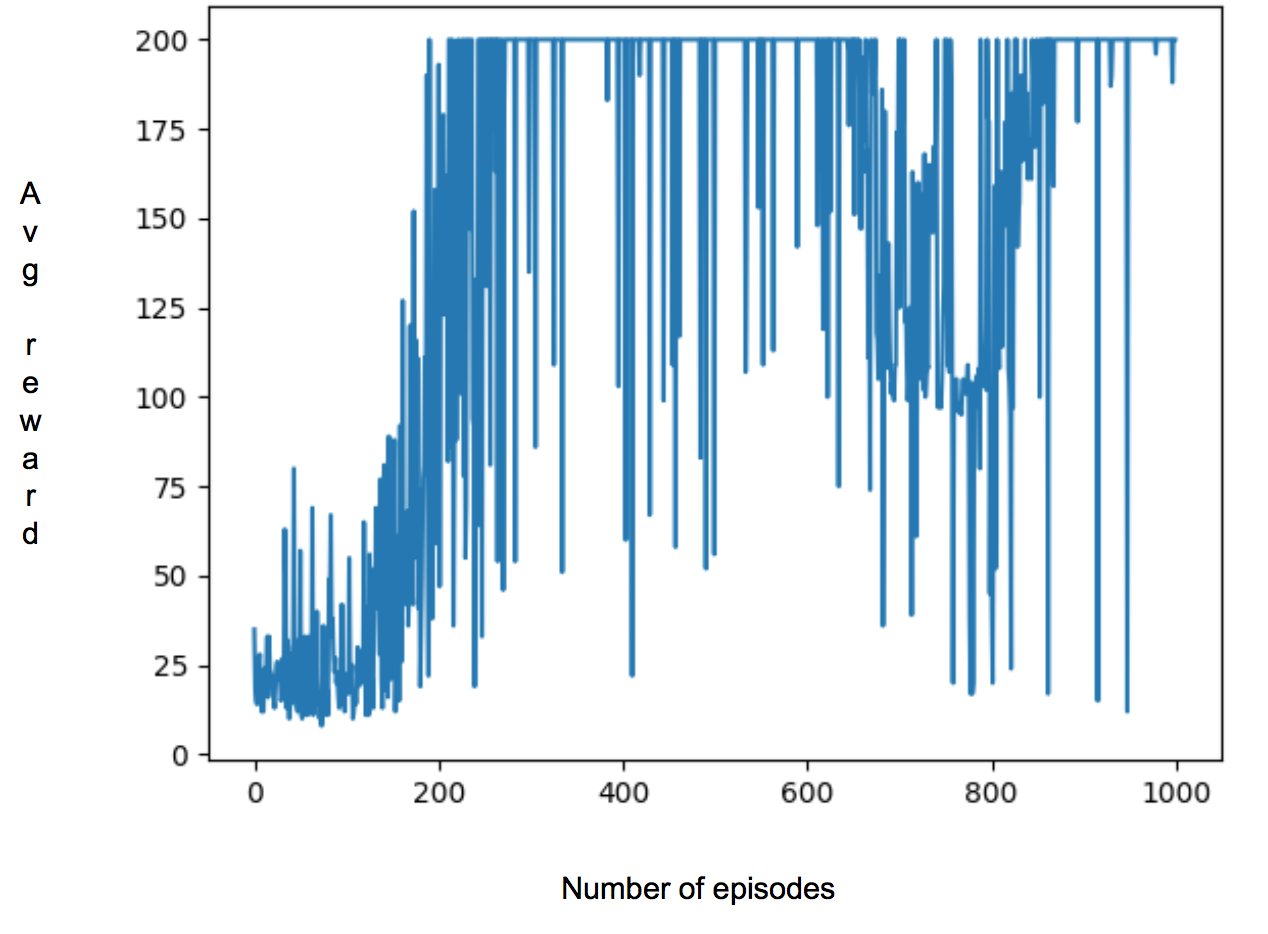
\includegraphics[width=0.4\textwidth]{images/e-greedy.png}
    \caption{
    Episode rewards for $\epsilon$-greedy strategy that had $\epsilon$ value over 0.1 for 1000 episodes. Decay value was 0.01 for the epsilon strategy in the formula 5.
    }
    \label{fig:e-greedy}
\end{figure}

\textbf{Different experience replay strategies} had also the results we expected. With a very small size of 2 model was not able to learn the task at all. With really high memory and batch size, it learned it really well. The only noticeable result was with the memory size of 1000. Intuitively we felt that 64 observations chosen randomly from 1000 would enough variation to break the strong correlation between close-by observations. This turned out to be not true like we can see from the figure \ref{fig:experience_replay}. Based on the figure model hasn't learned the task. It can achieve maximum score, but only for a short time. Then reward drops to almost zero. It seems that it learns a strategy, it utilizes it until it learns a completely new one. This cycle repeats and at least with 1000 episodes it hasn't learned any steady strategy.

\begin{figure}[H]
    \centering
    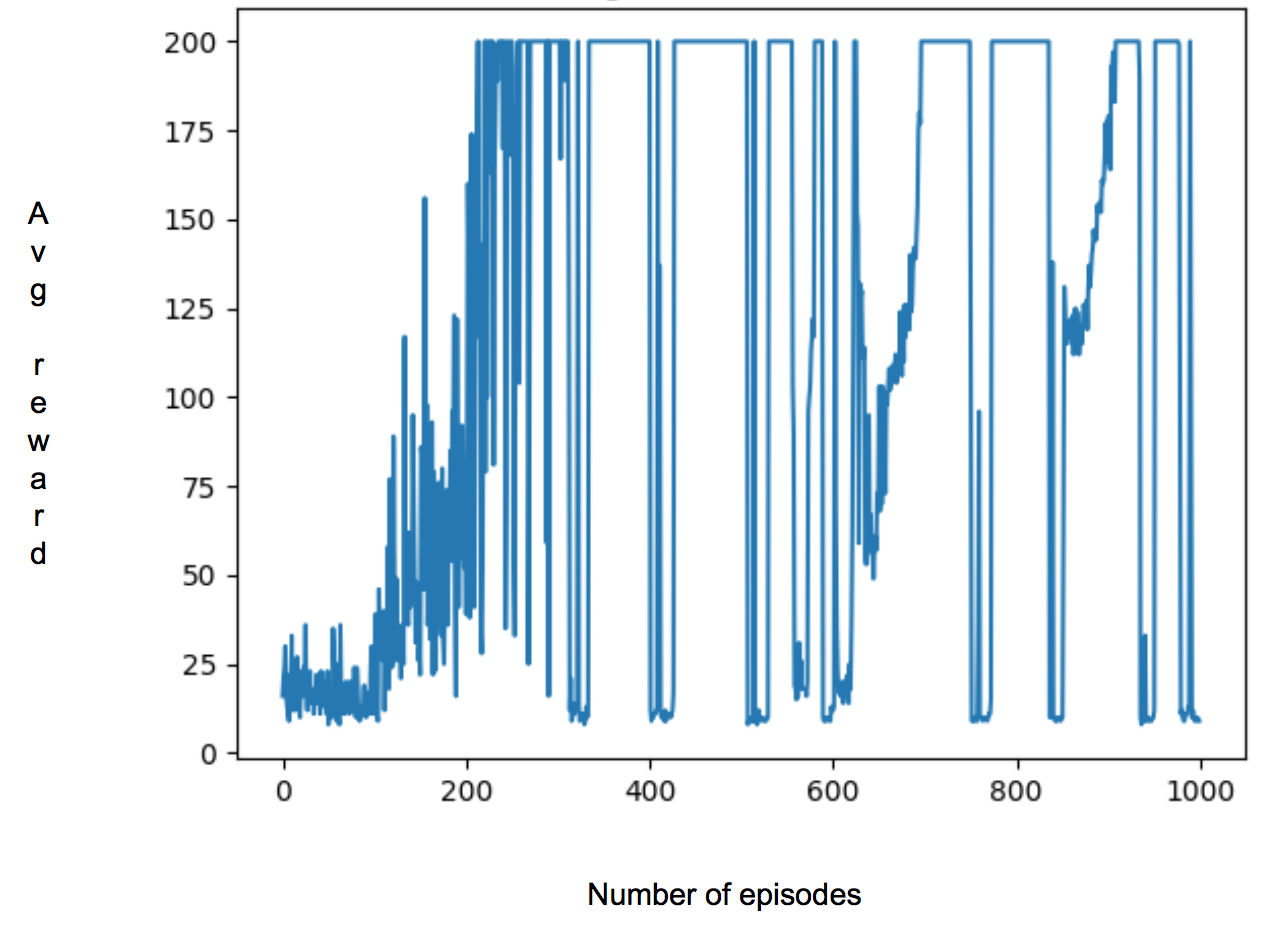
\includegraphics[width=0.4\textwidth]{images/experience_replay.png}
    \caption{
    Episode rewards when replay memory stored only the 1000 observations and had the batch size of 64.
    }
    \label{fig:experience_replay}
\end{figure}


  \section{Discussion}
  \label{sec:discussion}
  DQN turned out to be a very powerful method to learn Cart Pole. It was able to learn it quite quickly and small changes to the model didn't affect the learning that much. Only bigger changes in experience replay and $\epsilon$-greedy made it unstable. The same setup, unfortunately, didn't perform that well when the complexity of the task was increased from Cart Pole to Space Invaders.

We learned from this project that in modern reinforced learning the complex part is the network. Old reinforced algorithms work nicely when used correctly with modern deep learning methods.

To take this project further, we would implement a model with convolutional neural networks. Now when we understand every other part of the model, we can definitely implement that.


  %	REFERENCE LIST
  %----------------------------------------------------------------------------------------

  \bibliographystyle{IEEEtran}
  \bibliography{references}

\end{multicols} % One-column layout for the appendices
\pagebreak
\section{Appendix A: Dataset insights}
\label{appendix-a}
\input{appendix-a.tex}

\section{Appendix B: Pipeline}
\label{appendix-b}
\input{appendix-b.tex}

%----------------------------------------------------------------------------------------

\end{document}

%%% Local Variables:
%%% mode: latex
%%% TeX-master: t
%%% End:
